\section{задание: Классификация текстов}
\subsection{исходные данные}
\indent Входные данные: \textbf{Заголовки новостей} \\
\indent Категории (Классы): \textbf{[Politics,Sports,Tech,Finance]} \\
\indent Формат вывода: \textbf{JSON:{headline,topic}} \\
\newpage
\noindent Заголовки новостей (файл):
\begin{verbatim}
					 1) В МИД РФ призвали к «режиму тишины» вокруг переговоров
					по Украине. 2) Дмитриев: Мир восторжествует благодаря
					диалогу. 3) В Иране сообщают о новой волне студенческих
					протестов. 4) Расписание россиян на Олимпиаде-2026 в Милане
					22 февраля. 5) Журова о недопуске россиян на ЧМ: Им прекрасно
					достаются медали без наших спортсменов. 6) Ларионов не
					объявил игрокам СКА о своей скандальной поездке на финал
					ОИ-2026. 7) Фигуристы Аделия Петросян и Петр Гуменник заняли
					6-е места на Олимпиаде. 8) Лыжник Савелий Коростелев занял
					пятое место в олимпийском марафоне на 50 км. 9) Ученые NYU
					создали кристалл времени из полистироловых шариков и звуковых
					волн. 10) Минобрнауки запускает программу студенческих
					спутников. 11) Учёные зафиксировали отсутствие пятен на
					Солнце. 12) Вектор цифровизации смещается в сторону среднего
					бизнеса и городов. 13) Цифровой стресс-тест для
					промышленников. 14) Дёшево не будет: почему снижение ключевой
					ставки ударит по карманам россиян. 15) Сергей Миронов:
					«Вместо НДС на импорт нужны доступные кредиты для российских
					предприятий». 16) Россияне всё чаще выбирают безналичную
					оплату в магазинах. 17) Американская торговая палата
					выступила за смягчение ограничений. 18) Аналитик: укрепление
					рубля продолжится, устойчивый уровень — ниже 82 рублей за
					доллар. 19) Словакия выдвинула энергетический ультиматум
					Украине. 20) Депутат Журова прокомментировала недопуск
					российских фигуристов на ЧМ.
\end{verbatim}
\newpage
\subsection{базовый промпт}
\begin{verbatim}
					Классифицируй {ТЕМА} и выведи списком елементы,
					состоящие из номера предложения и его категории.
					Категории/Классы: {КАТЕГОРИИ}
\end{verbatim}
Запрос который предполагает просто классифицировать предложения из прикреплённого файла.
\subsection{журнал промпт-инжиниринга}
\noindent Промпт v1:
\begin{verbatim}
					Классифицируй Заголовки новостей и выведи списком елементы,
					состоящие из номера предложения и его категории.
					Категории/Классы: [Politics,Sports,Tech,Finance]
\end{verbatim}
\noindent Результат (YandexGPT):
\begin{figure}[H]
	\centering
	
\includegraphics[width=17cm]{z5/a1.png}
\end{figure}
\newpage
\noindent Анализ ошибок: модель верно классифицировала заголовки новостей. спорные заголовки 19 и 20 она отнесла к политическим. \\
Корректировка: добавить пример для каждой категории. \\
\newline
\noindent Промпт v2:
\begin{verbatim}
					Классифицируй Заголовки новостей и выведи списком елементы,
					состоящие из номера предложения и его категории.
					Категории/Классы: [Politics,Sports,Tech,Finance].
					Примеры:
						Текст: "1) В МИД РФ призвали к «режиму тишины» вокруг
					переговоров по Украине" -> 1) Politics
						Текст: "6) Ларионов не объявил игрокам СКА о своей
					скандальной поездке на финал ОИ-2026" -> 6) Sports
					 	Текст: "13) Цифровой стресс-тест для промышленников" ->
					13) Tech
						Текст: "18) Аналитик: укрепление рубля продолжится,
					устойчивый уровень — ниже 82 рублей за доллар" -> 18) Finance
\end{verbatim}
\noindent Результат (YandexGPT):
\begin{figure}[H]
	\centering
	
\includegraphics[width=13cm]{z5/b1.png}
\end{figure}
\noindent Анализ ошибок: модель (привязанная к данному региону) отказалась отвечать на запрос, так как обнаружила в запросе (связанным с данным регионом) паттерн, на который запрещено отвечать. \\
Корректировка: убрать примеры чтобы не задевать тригеры цензуры. \\
\newpage
\noindent Результат (DeepSeek):
\begin{figure}[H]
	\centering
	
\includegraphics[width=13cm]{z5/c1.png}
\end{figure}
\noindent Анализ ошибок: модель верно классифицировала заголовки новостей. спорные заголовки: 19 - Politics, и 20 - Sports \\
Корректировка: не требуется. \\
\newline
\noindent Промпт v3:
\begin{verbatim}
					Классифицируй Заголовки новостей и выведи списком елементы,
					состоящие из номера предложения и его категории.
					Категории/Классы: [Politics,Sports,Tech,Finance].
					Ответ должен быть ТОЛЬКО в формате JSON:{headline,topic},
					Не пиши ничего кроме структуры JSON.
\end{verbatim}
\newpage
\noindent Результат (YandexGPT):
\begin{figure}[H]
	\centering
	
\includegraphics[width=15cm]{z5/d1.png}
\end{figure}
\noindent Анализ ошибок: модель слишком буквально поняла запрос и вывела толко номер предложения. \\
Корректировка: изменить в запросе требуемый вывод. \\
\newpage
\noindent Результат (DeepSeek):
\begin{figure}[H]
	\centering
	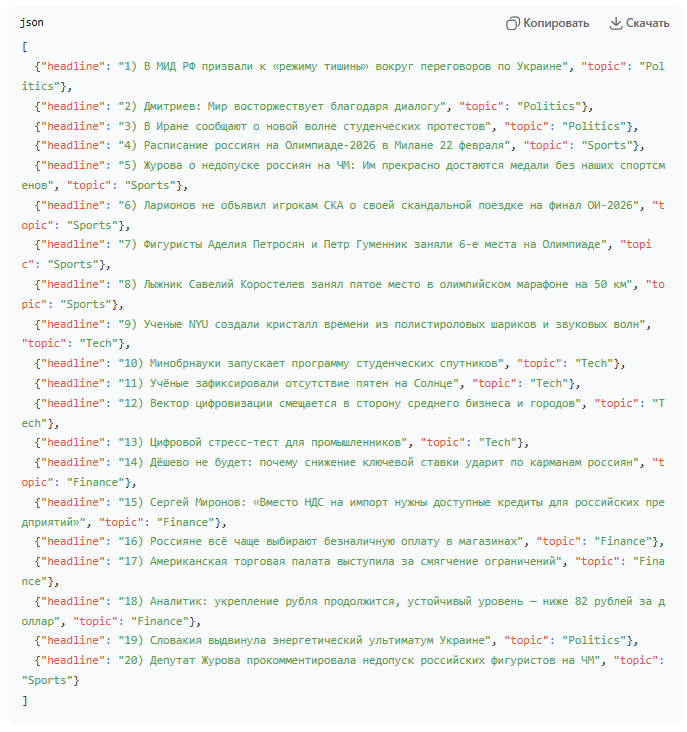
\includegraphics[width=15cm]{z5/e1.png}
\end{figure}
\noindent Анализ ошибок: модель правильно поняла задачу, но вывела заголовки с номером. \\
Корректировка: изменить в запросе требуемый вывод. \\
\newpage
\noindent Промпт v4:
\begin{verbatim}
					Классифицируй Заголовки новостей.
					Категории/Классы: [Politics,Sports,Tech,Finance].
					Ответ должен быть ТОЛЬКО в формате JSON:{headline,topic},
					Не пиши ничего кроме структуры JSON.
\end{verbatim}
\noindent Результат (YandexGPT):
\begin{figure}[H]
	\centering
	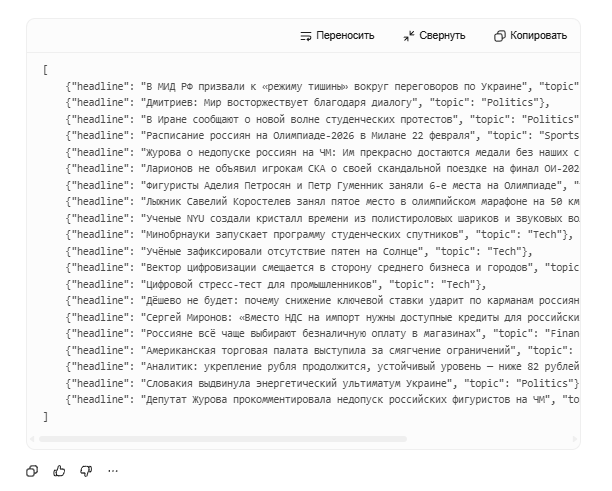
\includegraphics[width=14cm]{z5/f1.png}
\end{figure}
\noindent Анализ ошибок: модель выдала корректный JSON. \\
Корректировка: не требуется. \\
\newpage
\noindent Результат (DeepSeek):
\begin{figure}[H]
	\centering
	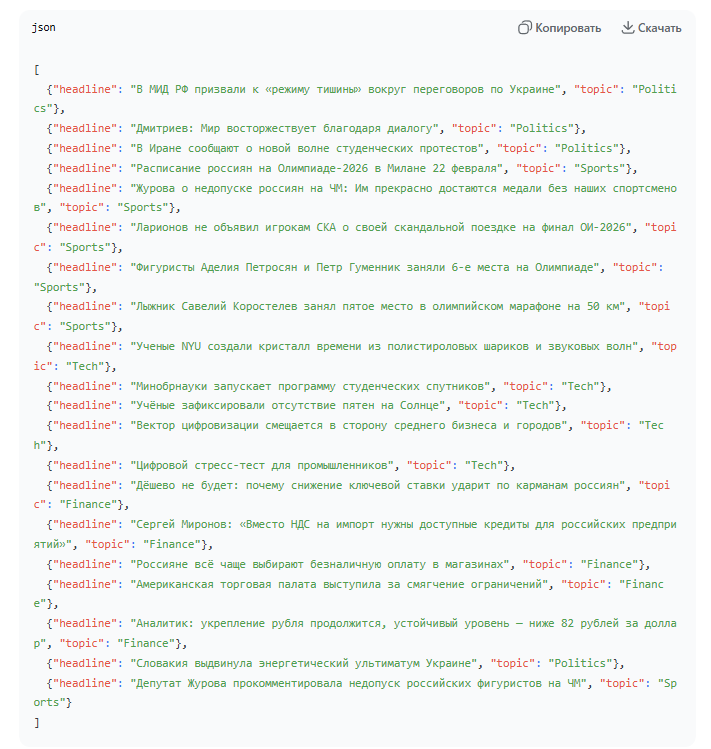
\includegraphics[width=14cm]{z5/g1.png}
\end{figure}
\noindent Анализ ошибок: модель выдала корректный JSON. \\
Корректировка: не требуется. \\
\newpage
\subsection{Сравнение моделей:}
\begin{table}[h!]
	\centering
	\begin{tabular}{|l|p{5cm}|p{5cm}|}
		\hline
		\textbf{Критерий} & \textbf{YandexGPT} & \textbf{DeepSeek} \\
		\hline
		Синтаксическая валидность & 5 & 5 \\
		\hline
		Схемное  соответствие & 5 & 5 \\
		\hline
		\textbf{Итог} & 5 & 5 \\
		\hline
	\end{tabular}
\end{table}
Каждая модель хооршо справилась с генерацией JSON, не смотря на региональные ограничения. У каждой модели свои региональные ограничения, которые стоит учитиывать.
\subsection{Финальный промпт:}
\begin{verbatim}
					Классифицируй {ТЕМА}.
					Категории/Классы: {КАТЕГОРИИ}.
					Ответ должен быть ТОЛЬКО в формате {ФОРМАТ},
					Не пиши ничего кроме структуры JSON.
\end{verbatim}
\subsection{Вывод по заданию:}
\indent В данном задании техника <<Обучение  на  примерах>> может предоставить более точный результат, потому что без неё нейросеть может неточно определять некоторые заголовки новостей.